\section{Un protocole d'échantillonnage aléatoire adaptatif}

\begin{frame}{Communication}{Propagation des modifications}

  Préserver la \textbf{cohérence à terme} des documents requière que tous les
  identifiants générés par la structure de séquences soient intégrés par tous
  les éditeurs.
  
  \vspace{0.5cm}
  
  Les éditeurs collaboratifs nécessitent un moyen de \textbf{communiquer} les
  changements effectués sur le document à tous les éditeurs impliqués dans
  l'édition.
  
  \vspace{0.5cm}

  \large
  \begin{itemize}
  \item [$\rightarrow$] \textbf{Dissémination d'information}
  \end{itemize}
  \vspace{0.5cm}
\end{frame}


\begin{frame}{Communication}{Contexte Web}
  
  \begin{minipage}{0.69\textwidth}
    Le contexte \textbf{Web} pousse à la \textbf{centralisation :}
    \begin{itemize}
    \item problèmes de \textbf{confidentialité}, \textbf{censure}, etc.
    \uncover<2->{\item problèmes de passage à l'échelle, notamment en \textbf{nombre de
        collaborateurs};}
    \uncover<3->{\item problèmes de \textbf{résilience} aux pannes.}
    \end{itemize}
  \end{minipage}
  \hfill
  \begin{minipage}{0.3\textwidth}
    
\includegraphics[width=0.7\textwidth]{img/www.png}
  \end{minipage}

  \vspace{0.75cm}
  

  \begin{minipage}{0.32\textwidth}
    \begin{center}
      \begin{tikzpicture}
        \node[visible on=<1-3>]
        {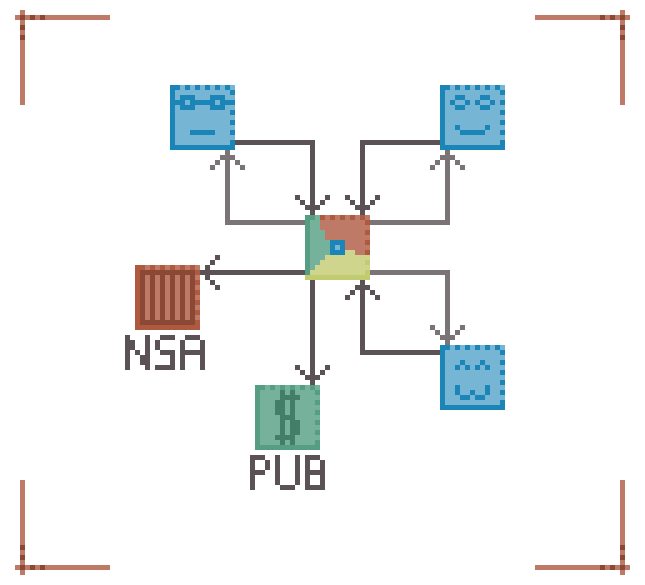
\includegraphics[width=0.95\textwidth]{img/centralizedethicproblems.png}};
      \end{tikzpicture}
    \end{center}
  \end{minipage}
  \begin{minipage}{0.32\textwidth}
    \begin{center}
      \begin{tikzpicture}
        \node[visible on=<2-3>]
        {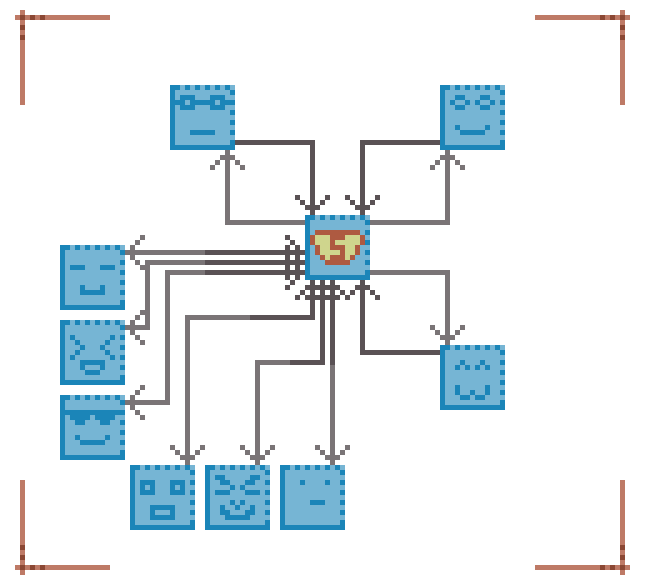
\includegraphics[width=0.95\textwidth]{img/centralizedcpuproblems.png}};
      \end{tikzpicture}
    \end{center}
  \end{minipage}
  \begin{minipage}{0.32\textwidth}
    \begin{center}
      \begin{tikzpicture}
        \node[visible on=<3-3>]
        {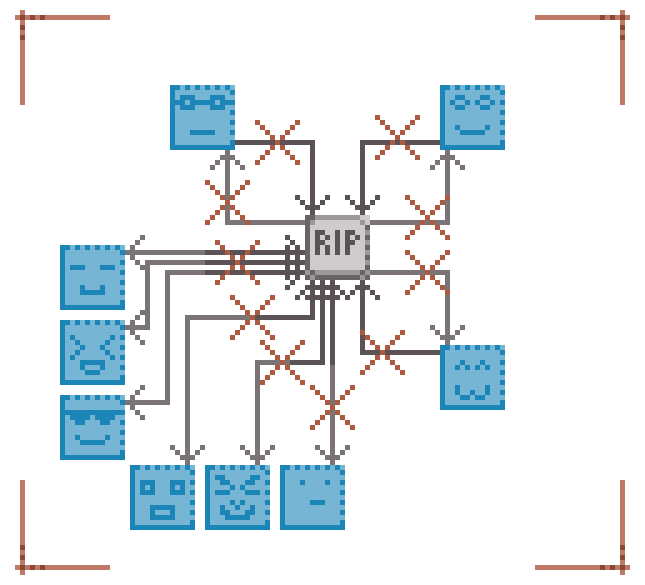
\includegraphics[width=0.95\textwidth]{img/centralizedscalabilityproblems.png}};
      \end{tikzpicture}        
    \end{center}
  \end{minipage}
\end{frame}

\begin{frame}{Communication}{Redécentralisation du Web}
  En \textbf{décentralisé}, la diffusion épidémique de messages constitue une
  manière efficace de disséminer l'information. Les messages parviennent à tous
  les pairs sans que ceux-ci ne connaissent tous les membres du réseau.

  \vspace{0.5cm}

  Fonctionnement : chaque pair possède une vue partielle du réseau.
  \begin{enumerate}
  \uncover<2->{\item un pair souhaitant diffuser un message l'envoie à sa vue partielle;}
  \uncover<3->{\item chaque pair recevant un tel message le diffuse à sa vue partielle;}
  \uncover<4->{\item condition d'arrêt : le message a déjà été reçu auparavant.}
  \end{enumerate}


  \begin{center}
    \begin{tikzpicture}[scale=1]

\newcommand\X{40pt}
\newcommand\Y{-15pt}

\draw[->] (0*\X, 0*\Y) -- (-5+1*\X,-3*\Y);
\draw[->](0*\X, 0*\Y) -- (-5+1*\X,-0*\Y);
\draw[->] (0*\X, 0*\Y) -- (-5+1*\X, 3*\Y);

% \only<2>\draw[->, very thick] (0*\X, 0*\Y) -- (-5+1*\X,-3*\Y);
% \only<2>\draw[->, very thick](0*\X, 0*\Y) -- (-5+1*\X,-0*\Y);
% \only<2>\draw[->, very thick] (0*\X, 0*\Y) -- (-5+1*\X, 3*\Y);


\draw[->] (1*\X, 3*\Y) -- (-5+2*\X, 4*\Y);
\draw[->] (1*\X, 3*\Y) -- (-5+2*\X, 3*\Y);
\draw[->] (1*\X, 3*\Y) -- (-5+2*\X, 2*\Y);

\draw[->] (1*\X, 0*\Y) -- (-5+2*\X, 1*\Y);
\draw[->] (1*\X, 0*\Y) -- (-5+2*\X, 0*\Y);
\draw[->] (1*\X, 0*\Y) -- (-5+2*\X,-1*\Y);

\draw[->] (1*\X,-3*\Y) -- (-5+2*\X,-2*\Y);
\draw[->] (1*\X,-3*\Y) -- (-5+2*\X,-3*\Y);
\draw[->] (1*\X,-3*\Y) -- (-5+2*\X,-4*\Y);

% \only<3>\draw[->, very thick] (1*\X, 3*\Y) -- (-5+2*\X, 4*\Y);
% \only<3>\draw[->, very thick] (1*\X, 3*\Y) -- (-5+2*\X, 3*\Y);
% \only<3>\draw[->, very thick] (1*\X, 3*\Y) -- (-5+2*\X, 2*\Y);

% \only<3>\draw[->, very thick] (1*\X, 0*\Y) -- (-5+2*\X, 1*\Y);
% \only<3>\draw[->, very thick] (1*\X, 0*\Y) -- (-5+2*\X, 0*\Y);
% \only<3>\draw[->, very thick] (1*\X, 0*\Y) -- (-5+2*\X,-1*\Y);

% \only<3>\draw[->, very thick] (1*\X,-3*\Y) -- (-5+2*\X,-2*\Y);
% \only<3>\draw[->, very thick] (1*\X,-3*\Y) -- (-5+2*\X,-3*\Y);
% \only<3>\draw[->, very thick] (1*\X,-3*\Y) -- (-5+2*\X,-4*\Y);


%\draw[<-, very thick, color=white] (5+1*\X, 5-3*\Y)to[out=90,in=140](-5+2*\X, 5-4*\Y);
%\draw[<-] (5+1*\X, 5-3*\Y)to[out=90,in=140](-5+2*\X, 5-4*\Y);
% \only<4>\draw[<-, very thick] (5+1*\X, 5-3*\Y)to[out=90,in=140](-5+2*\X, 5-4*\Y);
% \only<4>{\draw[fill=white, very thick] ( 2*\X, -4*\Y) node{$e_a$} +(-5pt,-5pt) rectangle +(5pt,5pt);}

%% ea --- ec
\draw[->](2*\X, -4*\Y) -- (3*\X, 5-4*\Y);
\draw[->](2*\X, -4*\Y) -- (3*\X, -5-4*\Y);
\draw[->](2*\X, -4*\Y) -- (3*\X, -0-4*\Y);
%\draw[->](2*\X, -4*\Y) -- (3*\X,  5-4*\Y);

\draw[->](2*\X, -3*\Y) -- (3*\X, -5-3*\Y);
\draw[->](2*\X, -3*\Y) -- (3*\X, -0-3*\Y);
\draw[->](2*\X, -3*\Y) -- (3*\X,  5-3*\Y);

\draw[->](2*\X, -2*\Y) -- (3*\X, -5-2*\Y);
\draw[->](2*\X, -2*\Y) -- (3*\X, -0-2*\Y);
\draw[->](2*\X, -2*\Y) -- (3*\X,  5-2*\Y);

%% ed --- ef
\draw[->](2*\X, -1*\Y) -- (3*\X, -5-1*\Y);
\draw[->](2*\X, -1*\Y) -- (3*\X, -0-1*\Y);
\draw[->](2*\X, -1*\Y) -- (3*\X,  5-1*\Y);

\draw[->](2*\X, -0*\Y) -- (3*\X, -5-0*\Y);
\draw[->](2*\X, -0*\Y) -- (3*\X, -0-0*\Y);
\draw[->](2*\X, -0*\Y) -- (3*\X,  5-0*\Y);

\draw[->](2*\X, 1*\Y) -- (3*\X, -5+1*\Y);
\draw[->](2*\X, 1*\Y) -- (3*\X, -0+1*\Y);
\draw[->](2*\X, 1*\Y) -- (3*\X,  5+1*\Y);

%% eg --- ei
\draw[->](2*\X, 2*\Y) -- (3*\X, -5+2*\Y);
\draw[->](2*\X, 2*\Y) -- (3*\X, -0+2*\Y);
\draw[->](2*\X, 2*\Y) -- (3*\X,  5+2*\Y);

\draw[->](2*\X, 3*\Y) -- (3*\X, -5+3*\Y);
\draw[->](2*\X, 3*\Y) -- (3*\X, -0+3*\Y);
\draw[->](2*\X, 3*\Y) -- (3*\X,  5+3*\Y);

\draw[->](2*\X, 4*\Y) -- (3*\X, -5+4*\Y);
\draw[->](2*\X, 4*\Y) -- (3*\X, -0+4*\Y);
\draw[->](2*\X, 4*\Y) -- (3*\X,  5+4*\Y);


%% ea --- ec
% \only<4>\draw[->, very thick](2*\X, -4*\Y) -- (3*\X, -5-4*\Y);
% \only<4>\draw[->, very thick](2*\X, -4*\Y) -- (3*\X, -0-4*\Y);
% %\only<4>\draw[->, very thick](2*\X, -4*\Y) -- (3*\X,  5-4*\Y);

% \only<4>\draw[->, very thick](2*\X, -3*\Y) -- (3*\X, -5-3*\Y);
% \only<4>\draw[->, very thick](2*\X, -3*\Y) -- (3*\X, -0-3*\Y);
% \only<4>\draw[->, very thick](2*\X, -3*\Y) -- (3*\X,  5-3*\Y);

% \only<4>\draw[->, very thick](2*\X, -2*\Y) -- (3*\X, -5-2*\Y);
% \only<4>\draw[->, very thick](2*\X, -2*\Y) -- (3*\X, -0-2*\Y);
% \only<4>\draw[->, very thick](2*\X, -2*\Y) -- (3*\X,  5-2*\Y);

% %% ed --- ef
% \only<4>\draw[->, very thick](2*\X, -1*\Y) -- (3*\X, -5-1*\Y);
% \only<4>\draw[->, very thick](2*\X, -1*\Y) -- (3*\X, -0-1*\Y);
% \only<4>\draw[->, very thick](2*\X, -1*\Y) -- (3*\X,  5-1*\Y);

% \only<4>\draw[->, very thick](2*\X, -0*\Y) -- (3*\X, -5-0*\Y);
% \only<4>\draw[->, very thick](2*\X, -0*\Y) -- (3*\X, -0-0*\Y);
% \only<4>\draw[->, very thick](2*\X, -0*\Y) -- (3*\X,  5-0*\Y);

% \only<4>\draw[->, very thick](2*\X, 1*\Y) -- (3*\X, -5+1*\Y);
% \only<4>\draw[->, very thick](2*\X, 1*\Y) -- (3*\X, -0+1*\Y);
% \only<4>\draw[->, very thick](2*\X, 1*\Y) -- (3*\X,  5+1*\Y);

% %% eg --- ei
% \only<4>\draw[->, very thick](2*\X, 2*\Y) -- (3*\X, -5+2*\Y);
% \only<4>\draw[->, very thick](2*\X, 2*\Y) -- (3*\X, -0+2*\Y);
% \only<4>\draw[->, very thick](2*\X, 2*\Y) -- (3*\X,  5+2*\Y);

% \only<4>\draw[->, very thick](2*\X, 3*\Y) -- (3*\X, -5+3*\Y);
% \only<4>\draw[->, very thick](2*\X, 3*\Y) -- (3*\X, -0+3*\Y);
% \only<4>\draw[->, very thick](2*\X, 3*\Y) -- (3*\X,  5+3*\Y);

% \only<4>\draw[->, very thick](2*\X, 4*\Y) -- (3*\X, -5+4*\Y);
% \only<4>\draw[->, very thick](2*\X, 4*\Y) -- (3*\X, -0+4*\Y);
% \only<4>\draw[->, very thick](2*\X, 4*\Y) -- (3*\X,  5+4*\Y);



\draw[fill=white] ( 0*\X, 0*\Y) node{$e$} +(-5pt,-5pt) rectangle +(5pt,5pt);
% \only<2>{\draw[fill=white, very thick] ( 0*\X, 0*\Y) node{$e$} +(-5pt,-5pt) rectangle +(5pt,5pt);}

\draw[fill=white] ( 1*\X,-3*\Y) node{$e_1$} +(-5pt,-5pt) rectangle +(5pt,5pt);
\draw[fill=white] ( 1*\X, 0*\Y) node{$e_2$} +(-5pt,-5pt) rectangle +(5pt,5pt);
\draw[fill=white] ( 1*\X, 3*\Y) node{$e_3$} +(-5pt,-5pt) rectangle +(5pt,5pt);

% \only<3>{\draw[fill=white, very thick] ( 1*\X,-3*\Y) node{$e_1$} +(-5pt,-5pt) rectangle +(5pt,5pt);}
% \only<3>{\draw[fill=white, very thick] ( 1*\X, 0*\Y) node{$e_2$} +(-5pt,-5pt) rectangle +(5pt,5pt);}
% \only<3>{\draw[fill=white, very thick] ( 1*\X, 3*\Y) node{$e_3$} +(-5pt,-5pt) rectangle +(5pt,5pt);}


\draw[fill=white] ( 2*\X, -4*\Y) node{$e_a$} +(-5pt,-5pt) rectangle +(5pt,5pt);
\draw[fill=white] ( 2*\X, -3*\Y) node{$e_b$} +(-5pt,-5pt) rectangle +(5pt,5pt);
\draw[fill=white] ( 2*\X, -2*\Y) node{$e_c$} +(-5pt,-5pt) rectangle +(5pt,5pt);

\draw[fill=white] ( 2*\X, -1*\Y) node{$e_d$} +(-5pt,-5pt) rectangle +(5pt,5pt);
\draw[fill=white] ( 2*\X,  0*\Y) node{$e_e$} +(-5pt,-5pt) rectangle +(5pt,5pt);
\draw[fill=white] ( 2*\X,  1*\Y) node{$e_f$} +(-5pt,-5pt) rectangle +(5pt,5pt);

\draw[fill=white] ( 2*\X,  2*\Y) node{$e_g$} +(-5pt,-5pt) rectangle +(5pt,5pt);
\draw[fill=white] ( 2*\X,  3*\Y) node{$e_h$} +(-5pt,-5pt) rectangle +(5pt,5pt);
\draw[fill=white] ( 2*\X,  4*\Y) node{$e_i$} +(-5pt,-5pt) rectangle +(5pt,5pt);

% \only<4>{\draw[fill=white, very thick] ( 2*\X, -4*\Y) node{$e_a$} +(-5pt,-5pt) rectangle +(5pt,5pt);}
% \only<4>{\draw[fill=white, very thick] ( 2*\X, -3*\Y) node{$e_b$} +(-5pt,-5pt) rectangle +(5pt,5pt);}
% \only<4>{\draw[fill=white, very thick] ( 2*\X, -2*\Y) node{$e_c$} +(-5pt,-5pt) rectangle +(5pt,5pt);}

% \only<4>{\draw[fill=white, very thick] ( 2*\X, -1*\Y) node{$e_d$} +(-5pt,-5pt) rectangle +(5pt,5pt);}
% \only<4>{\draw[fill=white, very thick] ( 2*\X,  0*\Y) node{$e_e$} +(-5pt,-5pt) rectangle +(5pt,5pt);}
% \only<4>{\draw[fill=white, very thick] ( 2*\X,  1*\Y) node{$e_f$} +(-5pt,-5pt) rectangle +(5pt,5pt);}

% \only<4>{\draw[fill=white, very thick] ( 2*\X,  2*\Y) node{$e_g$} +(-5pt,-5pt) rectangle +(5pt,5pt);}
% \only<4>{\draw[fill=white, very thick] ( 2*\X,  3*\Y) node{$e_h$} +(-5pt,-5pt) rectangle +(5pt,5pt);}
% \only<4>{\draw[fill=white, very thick] ( 2*\X,  4*\Y) node{$e_i$} +(-5pt,-5pt) rectangle +(5pt,5pt);}



\end{tikzpicture}
  \end{center}

\end{frame}

\begin{frame}{Communication}{Possible grâce à WebRTC, mais\ldots}

  \begin{itemize}
  \item [$\rightarrow$] Récemment rendu possible grâce à WebRTC : un navigateur
    peut devenir \textbf{à la fois client et serveur}.
    \begin{itemize}
    \item Les nœuds n'ont \textbf{ni adresses ni routes}, les connexions sont
      plus \textbf{coûteuses} et sujettes aux \textbf{defaillances} que sur
      réseau IP;
    \item Les navigateurs Web fonctionnent sur des outils aux \textbf{capacités
        hétérogènes et parfois limités};
    \item Web expose aux \textbf{pics soudains de popularité.}
    \end{itemize}
  \end{itemize}
  

\end{frame}

